\documentclass{report}
\usepackage[spanish]{babel}
\usepackage[utf8]{inputenc}
\usepackage{graphicx, longtable, float, titlesec, hyperref, enumitem, dingbat}
\usepackage[dvipsnames]{xcolor}
\usepackage[margin=2.75cm]{geometry}

\hypersetup{
    hidelinks = true
}

\titleformat{\chapter}[display]
  {\normalfont\bfseries}{}{0pt}{\Huge\thechapter.\space}

\titleformat{name=\chapter,numberless}[display]
  {\normalfont\bfseries}{}{0pt}{\Huge}

\titlespacing*{\chapter}{0pt}{-50pt}{20pt}


\begin{document}
    \begin{titlepage}
        \centering
        
\includegraphics[width=0.6\textwidth]{./img/logo.jpg}\\
        \vspace{1cm}
        \LARGE Gestión de proyectos\\
        \vspace{0.5cm}
        \Large Ingeniería Informática de Gestión y Sistemas de Información\\
        \vspace{3cm}
        \Huge PromoIng Civil UPV/EHU\\
        \vspace{2.5cm}
        \Large Autor:\\
        \vspace{0.2cm}
        \large Xabier Gabiña\\
        \large Endika Postigo\\
        \large Xabier Badiola\\
        \large Ander Gorocica\\
        \large Asier Larrazabal\\
        \large Pablo Leclercq\\
        \vfill
        \today
    \end{titlepage}
    \tableofcontents
    \listoffigures
    \listoftables
    \chapter{Introducción}
        \section{Introducción del Proyecto}
            \paragraph*{}
            Este documento detalla la propuesta solicitada por la persona responsable para promocionar las titulaciones de la Escuela de Ingeniería de Bilbao para el desarrollo de un vídeo promocional y una plataforma web. El objetivo es destacar la titulación de Ingeniería Civil, subrayando sus beneficios únicos, infraestructura y oportunidades. Además, la plataforma web mostrará un video sobre dicha titulación y servirá para recoger datos de contacto de estudiantes potenciales e incluirá la organización de un sorteo entre los participantes, ofreciendo material corporativo de la universidad como incentivo.
        \section{Propósito del Proyecto}
            \paragraph*{}
            El propósito de este proyecto es elaborar un video promocional y desarrollar una página web que exponga de manera atractiva y concisa las características de la titulación de Ingeniería Civil de la Escuela de Ingeniería de Bilbao, incluyendo los objetivos educativos, infraestructura, y las oportunidades de prácticas y proyectos. Proporcione una manera directa y sencilla para que los interesados dejen sus datos de contacto a través de la plataforma web, facilitando así la recolección de información. Además, se incluirá en la plataforma un sorteo de material corporativo de la universidad entre los participantes que completen el formulario de contacto.
        \section{Asociaciones y Ámbito de Aplicación}
            \paragraph*{}
            Este proyecto se realiza a petición de la persona encargada de la promoción de las titulaciones en la Escuela de Ingeniería de Bilbao y está diseñado para soportar la promoción de sus programas académicos. La plataforma web contendrá el video promocional y será accesible en todos los navegadores, asegurando que el público objetivo pueda acceder fácilmente a la información y participar en el sorteo.
        \section{Contexto de Negocio}
            \paragraph*{}
            El proyecto se enfoca en proporcionar herramientas digitales promocionales específicas para la Escuela de Ingeniería de Bilbao, orientadas a atraer a estudiantes de último año de bachillerato y profesionales jóvenes interesados en las titulaciones ofrecidas, en nuestro caso la Ingeniería Civil.. Responde a la necesidad de la escuela de resaltar los puntos fuertes de sus programas y de facilitar la recogida de datos de posibles candidatos, promoviendo así un mayor interés tanto a nivel nacional como internacional. La inclusión de un sorteo busca añadir un incentivo adicional para el registro de datos en la plataforma.
        \section{Definiciones, Acrónimos y Abreviaturas}
            \paragraph*{}
            \begin{itemize}
                \item \textbf{UPV/EHU:} Universidad del País Vasco/Euskal Herriko Unibertsitatea.
                \item \textbf{DOP:} Documento de Planificación.
                \item \textbf{PromoIng Civil UPV/EHU:} Proyecto de promoción de la titulación de Ingeniería Civil de la UPV/EHU.
                \item \textbf{SMART:} Es un acrónimo en inglés que se utiliza para definir objetivos específicos, medibles, alcanzables, relevantes y con un tiempo determinado.
            \end{itemize}
    \chapter{Descripción del proyecto}
        \section{Descripción del Proyecto}
            \paragraph*{}
            El proyecto PromoIng Civil UPV/EHU es una iniciativa encargada por la persona responsable de promocionar las titulaciones de la Escuela de Ingeniería de Bilbao, perteneciente a la Universidad del País Vasco / Euskal Herriko Unibertsitatea (UPV/EHU). Este proyecto integra el desarrollo de un video promocional y una plataforma web, destinados a resaltar las ventajas y oportunidades de estudiar la titulación de Ingeniería Civil en una de las instituciones más reconocidas de la región. Un aspecto distintivo de la plataforma web será la inclusión de un sorteo entre los interesados que proporcionen sus datos, ofreciendo material corporativo de la universidad como premio.
        \section{Problema que Resuelve}
            \paragraph*{}
            En un contexto de creciente competencia educativa, la UPV/EHU enfrenta el reto de mantener y diversificar su matrícula. El proyecto PromoIng Civil UPV/EHU surge como respuesta a la necesidad de mejorar la visibilidad y efectividad de las comunicaciones sobre la titulación de Ingeniería Civil. Al presentar de manera más atractiva esta titulación a potenciales estudiantes, tanto a nivel local como internacional, y facilitar la recopilación de datos de los interesados, el proyecto busca fortalecer la comunidad universitaria.
        \section{Valor del Desarrollo}
            \paragraph*{}
            La importancia de desarrollar PromoIng Civil UPV/EHU reside en varios aspectos clave:
            \begin{itemize}
                \item \textbf{Fortalecimiento de la Identidad Institucional:} La asociación directa del proyecto con la UPV/EHU destaca el prestigio y la calidad de la universidad, reforzando su imagen como líder en la educación en ingeniería.
                \item \textbf{Mejora de la Estrategia de Comunicación:} Mediante el uso de herramientas digitales y contenido atractivo, el proyecto facilita la comunicación de las características únicas y beneficios de la titulación de Ingeniería Civil, resonando con las expectativas de los estudiantes actuales.
                \item \textbf{Aumento de la Visibilidad y Alcance:} Se busca mejorar la posición de la Escuela de Ingeniería de Bilbao y de la UPV/EHU en el ámbito nacional e internacional como referentes en estudios de ingeniería.
                \item \textbf{Optimización del Proceso de Reclutamiento:} La plataforma web ofrecerá un canal directo y eficiente para interactuar con los interesados, facilitando el proceso de admisión y aumentando las tasas de conversión de interesados a estudiantes matriculados.
            \end{itemize}
            En conclusión, el proyecto PromoIng Civil UPV/EHU no solo eleva la visibilidad de una titulación específica sino que también contribuye al fortalecimiento de la marca UPV/EHU como institución líder en educación superior, especialmente en ingeniería. Este esfuerzo se alinea con los objetivos estratégicos de la universidad de atraer talento y fomentar la innovación y la excelencia académica en el País Vasco y más allá, incluyendo el sorteo como un incentivo adicional para la participación en la plataforma web.
    \chapter{Objetivos del proyecto}
        \section{Desarrollo del Proyecto PromoEng Civil UPV/EHU}
            \paragraph*{}
            El proyecto PromoEng Civil UPV/EHU tiene como fin el desarrollo de una plataforma web accesible y la producción de un video promocional integrado en dicha plataforma. Este enfoque busca maximizar la visibilidad y el atractivo de la titulación de Ingeniería Civil de la Escuela de Ingeniería de Bilbao, UPV/EHU. Los objetivos son:
            \begin{itemize}
                \item Desarrollar una plataforma web accesible y producir un video promocional de 3 minutos para aumentar la visibilidad y el atractivo de la titulación de Ingeniería Civil de la Escuela de Ingeniería de Bilbao, UPV/EHU.
                \item Producir un video que incluya testimonios, vistas de instalaciones y descripciones de oportunidades profesionales, integrándolo de manera destacada en la plataforma web para asegurar su visibilidad. La plataforma debe incluir secciones para información del programa, contacto, y el video promocional, además de un sistema para la recopilación y gestión eficiente de datos de contacto.
                \item Utilizar el video como herramienta clave para aumentar el interés por la titulación, complementando la información disponible en la plataforma web. Proporcionar un recurso completo y accesible para aumentar las solicitudes de información y admisión.
                \item Completar el video y su integración en la plataforma web en un plazo de 4 meses desde el inicio del proyecto. Finalizar el desarrollo, pruebas y lanzamiento de la plataforma web en el mismo período. Completar las pruebas y ajustes necesarios antes del lanzamiento oficial de la plataforma y el video.
            \end{itemize}
    \chapter{Arquitectura}
        \paragraph*{}
        Hemos decidido utilizar una arquitectura Web y una plataforma llamada Docker para realizar este proyecto. Docker sigue una estructura basada en contenedores y los utiliza para encapsular y distribuir aplicaciones. Dentro de este proyecto vamos a incluir un contenedor para desplegar la página web, otro para el reproductor de youtube y otro para el formulario de Google Forms, que este tendrá una base de datos. La página web tendrá la siguiente estructura:
        \begin{itemize}
            \item Un video donde resume la información que contiene la pantalla de inicio.
            \item Información relevante sobre el grado de Ingeniería Civil, por ejemplo, las salidas que tiene el grado, los puestos de trabajo en los que pueden trabajar en un futuro al terminarlo, opiniones sobre los alumnos que han cursado este grado.
            \item Un formulario donde se recoge información de interés sobre los interesados en cursar el grado, por ejemplo, los estudios actuales, la edad, el curso que está realizando, si está realizando un bachiller o una FP, quien rellena la encuesta (familiar, el propio alumno…). Además, se van a sortear dos mochilas de la UPV/EHU entre las personas que rellenen la encuesta (el sorteo se realizará de manera aleatoria y manual).
        \end{itemize}
        
        Dentro de la base de datos de Google Forms se guardará toda la información relativa a los usuarios que rellenen la encuesta de la página web.\\
        \clearpage
        La arquitectura de este sistema web funciona de la siguiente manera:
        \begin{itemize}
            \item El usuario accede a la página web desde su navegador.
            \item La página web esta desplegada en un cluster Kubernetes corriendo en Google Cloud que asegura la disponibilidad de la página web.
            \item Dicho cluster esta corriendo un 'Pod' con la imagen Docker de la página web de esta forma se consigue que la web sea facilmente escalable.
            \item La página web carga elementos de Youtube y Google Forms mediante iFrames además de los elementos propios y los muestra mediante el navegador al usuario.
        \end{itemize}
        \begin{figure}[H]
            \centering
            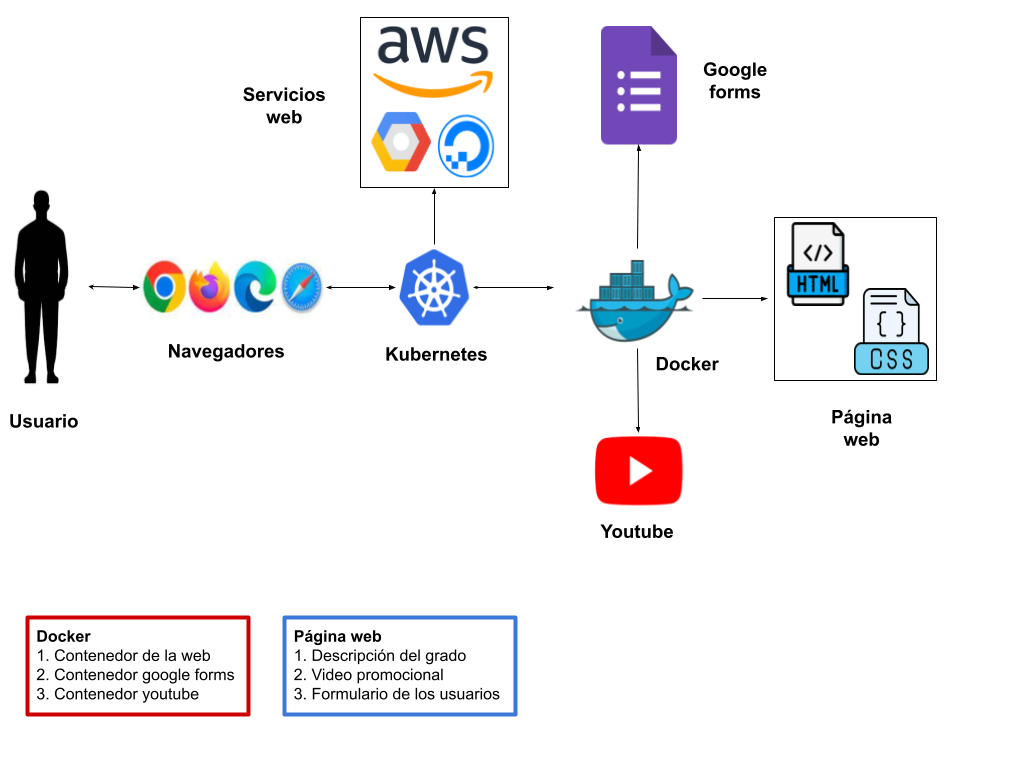
\includegraphics[width=0.8\textwidth]{./img/arquitectura.png}
            \caption{Arquitectura del sistema}
        \end{figure}
    \chapter{Herramientas}
        \section*{Git}
            Git es un sistema de control de versiones distribuido de código abierto y gratuito diseñado para manejar todo, desde proyectos pequeños hasta muy grandes, con velocidad y eficiencia. Lo utilizaremos para controlar las versiones del código fuente de la página web.
        \section*{GitHub}
            GitHub es una plataforma de desarrollo colaborativo para alojar proyectos utilizando el sistema de control de versiones Git. Lo utilizaremos para alojar el código fuente de la página web junto con la documentación del proyecto
        \section*{LibreOffice}
            LibreOffice es una suite ofimática de codigo abierto que incluye programas para el procesamiento de texto, hojas de cálculo, presentaciones, bases de datos y dibujos. Lo utilizaremos para la redacción de la documentacion.
        \section*{LaTeX}
            LaTeX es un sistema de composición de textos, orientado a la creación de documentos escritos que presenten una alta calidad tipográfica. Lo utilizaremos para la redacción de la documentacion.
        \section*{Apache HTTP Server}
            Apache HTTP Server es un servidor web HTTP de código abierto multiplataforma que nos servira para desarrollar nuestra página web.
        \section*{Docker}
            Docker es un proyecto de código abierto que automatiza el despliegue de aplicaciones dentro de contenedores de software, proporcionando una capa adicional de abstracción y automatización de virtualización a nivel de sistema operativo en Linux. Utilizaremos Docker para desplegar nuestra página web en un contenedor.
        \section*{Kubernetes}
            Kubernetes es un sistema de código abierto para la automatización del despliegue, escalado y manejo de aplicaciones en contenedores originalmente diseñada por Google. La usaremos para desplegar nuestra imagen Docker en un cluster de Google Cloud.
        \section*{VSCode}
            Visual Studio Code es un editor de código fuente desarrollado por Microsoft para Windows, Linux y macOS. Lo utilizaremos para la programación de la página web.
        \section*{Google Cloud Platform}
            Google Cloud Platform es una suite de servicios en la nube que se ejecutan en la misma infraestructura que Google utiliza internamente para sus productos de usuario final, como Google Search y YouTube. Junto con un conjunto de herramientas de administración, seguridad y desarrollo, Google Cloud Platform proporciona una serie de servicios como es el caso de Kubernete Engine.
        \section*{Google Forms}
            Google Forms es una herramienta de Google que nos permite crear encuestas y cuestionarios de manera sencilla y rápida. Lo utilizaremos para recoger información de los interesados en cursar el grado de Ingeniería Civil.
        \section*{Youtube}
            Youtube es una plataforma de videos en la que los usuarios pueden subir, compartir y ver videos. Lo utilizaremos para alojar el video promocional de la página web.
        \section*{GanttProject}
            GanttProject es una herramienta de código abierto para la creación de diagramas de Gantt y la gestión de proyectos. Lo utilizaremos para la planificación temporal del proyecto.
    \chapter{Alcance del proyecto} %TODO
            \subsection{Ciclo de vida}
                \paragraph*{}
                Para el desarrollo de este proyecto hemos decidido utilizar un ciclo de vida adaptativo o ágil. Las actividades de desarrollo se completarán una tras otra. Las actividades de prueba solo ocurrirán después de que todas las actividades de desarrollo se hayan completado.  Tomaremos el siguiente orden de ciclo:
                \begin{figure}[H]
                    \centering
                    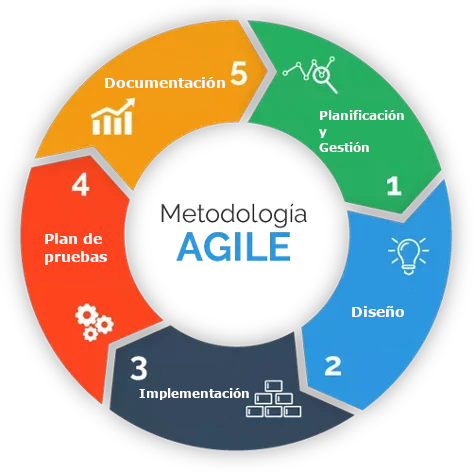
\includegraphics[width=0.5\textwidth]{./img/ciclo_vida.png}
                    \caption{Ciclo de vida del proyecto}
                \end{figure}
                Una de las razones por la que hemos elegido este modelo de ciclo de vida es que los equipos trabajan en ciclos cortos de desarrollo y además se adaptan a los cambios propuestos por el cliente a medida que surgen, pudiendo variar así la planificación y la gestión del proyecto en cualquier momento.
            \clearpage
            \subsection{Fases del proyecto}
                \textbf{EDT}
                \begin{figure}[H]
                    \centering
                    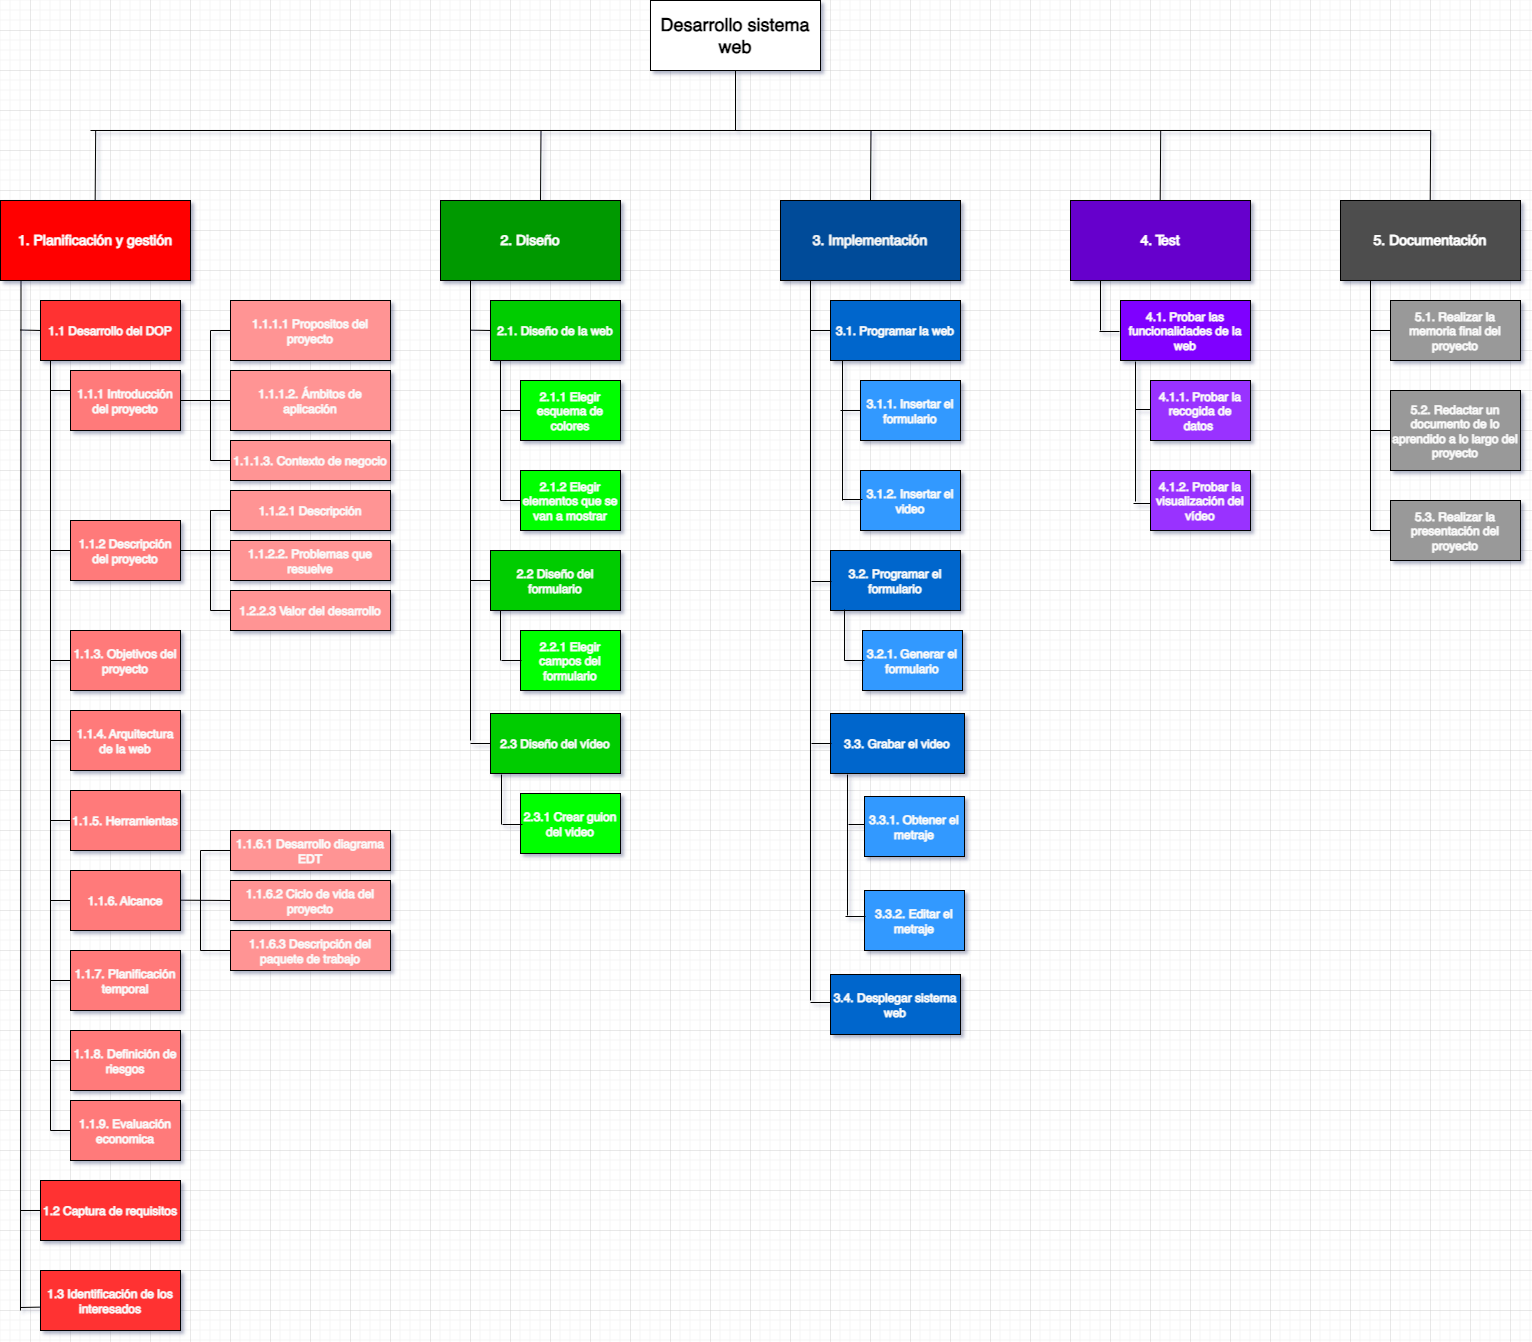
\includegraphics[width=0.8\textwidth]{./img/edt.png}
                    \caption{EDT del proyecto}
                \end{figure}
            \clearpage
        \section{Planificación y Gestión}
        \section{Diseño}
        \section{Implementación}
        \section{Plan de pruebas}
        \section{Documentación}
    \chapter{Planificación temporal} %TODO
    \chapter{Riesgos}
        \begin{center}
            \begin{longtable}{|p{6cm}|p{6cm}|}
                \hline
                \textbf{Descripción} & Que un agente externo mediante una vulnerabilidad de seguridad pueda realizar acciones no autorizadas en la página web.\\
                \hline
                \textbf{Prevención} & Realizar pruebas de seguridad en la página web.\\
                \hline
                \textbf{Plan de contingencia} & Parchear la vulnerabilidad y realizar una auditoría de seguridad en la página web.\\
                \hline
                \textbf{Probabilidad} & Media\\
                \hline
                \textbf{Impacto} & Muy alto\\
                \hline
                \caption{Vulnerabilidades de seguridad}
            \end{longtable}
        \end{center}
        \begin{center}
            \begin{longtable}{|p{6cm}|p{6cm}|}
                \hline
                \textbf{Descripción} & Perder toda o parte de la información almacenada en Google Forms.\\
                \hline
                \textbf{Prevención} & Guardar copias de seguridad de la información en un lugar seguro.\\
                \hline
                \textbf{Plan de contingencia} & Utilizar las copias de seguridad para recuperar la información perdida.\\
                \hline
                \textbf{Probabilidad} & Baja\\
                \hline
                \textbf{Impacto} & Muy alto\\
                \hline
                \caption{Perdida de información}
            \end{longtable}
        \end{center}
        \begin{center}
            \begin{longtable}{|p{6cm}|p{6cm}|}
                \hline
                \textbf{Descripción} & Asegurar que los datos recogidos en Google Forms no sean accesibles por terceros.\\
                \hline
                \textbf{Prevención} & Cifrar la conexion con la web y usar contraseña seguras con 2FA en la cuenta de Google.\\
                \hline
                \textbf{Plan de contingencia} & Generar nuevos certificados para la web y nueva contraseña para la cuenta de Google.\\
                \hline
                \textbf{Probabilidad} & Baja\\
                \hline
                \textbf{Impacto} & Medio\\
                \hline
                \caption{Seguridad de datos}
            \end{longtable}
        \end{center}
        \clearpage
        \begin{center}
            \begin{longtable}{|p{6cm}|p{6cm}|}
                \hline
                \textbf{Descripción} & Asegurar que la página web no utiliza ningun elemento incompatible con los navegadores actuales.\\
                \hline
                \textbf{Prevención} & Probar de forma periodica la página web en los navegadores más utilizados.\\
                \hline
                \textbf{Plan de contingencia} & Modificar la página web para que sea compatible con los navegadores actuales en el menor tiempo posible.\\
                \hline
                \textbf{Probabilidad} & Muy baja\\
                \hline
                \textbf{Impacto} & Alto\\
                \hline
                \caption{Compatibilidad de navegadores}
            \end{longtable}
        \end{center}
        \begin{center}
            \begin{longtable}{|p{6cm}|p{6cm}|}
                \hline
                \textbf{Descripción} & Asegurar que la página web escala correctamente en función del número de usuarios y que no se producen caidas.\\
                \hline
                \textbf{Prevención} & Realizar pruebas de carga en la página web.\\
                \hline
                \textbf{Plan de contingencia} & Aumentar la capacidad de la página web mediante la creación de más contenedores (escalado horizontal).\\
                \hline
                \textbf{Probabilidad} & Alta\\
                \hline
                \textbf{Impacto} & Alto\\
                \hline
                \caption{Problemas de escalabilidad}
            \end{longtable}
        \end{center}
    \chapter{Evaluación económica} %TODO
    \chapter*{Anexo} %TODO
        \section*{Paquetes de trabajo} %TODO
\end{document}